\chapter{物種想要起源但是物種不說}
\chapterauthor{高語儂}

\section{演化的定義}
地球上的生物,一直在改變。 \\
\subsection{複習下達爾文演化}
\begin{enumerate}
\item \textbf{變異:}
物種間,其性狀在個體存在差異
\item \textbf{過度繁殖:}
族群的個體數過多時,其生活所需的食物、水或空間便感不足。
\item \textbf{生存競爭:}
個體為了生存,彼此間會搶奪資源
\item \textbf{適者生存:}
成功的個體生存下來,並產生後代子孫。 
\end{enumerate}

\subsection{歷史小故事}
\begin{enumerate}
\item 達爾文在小獵犬之行後快30年(1859)才出版物種起源
\item 科學界在1870年代正式接受演化是事實。
\end{enumerate}

\section{演化的基本單位}
生物學將生命分成不同階層,從細胞、組織、器官到個體,並進一步形成族群、群集、生態系最後構成生物圈,那麼,\textbf{在研究演化時,科學家們通常會關注生命的哪個層面呢?why?}

事實上,演化可分為「微演化」和「巨演化」,今天我們要詳細介紹的是\underline{\hspace{6em}} 
微演化關注的是一個\underline{\hspace{4em}}中,等位基因頻率的變化。
巨演化通常指更大尺度的變化,例如新器官的生成,以及新物種的出現。

補充:微演化的分類
\begin{enumerate}
\item \textbf{天擇:}因為環境,而讓帶有特定「表型」的個體有生存優勢。
\item \textbf{基因漂變:}基因分布隨機的改變,例如:基因突變、瓶頸效應、創始者效應
\item \textbf{基因流動:}不同族群間的基因交換,例如:台灣人與日本人結婚
\end{enumerate}
\fbox{簡短名詞解釋}
\begin{enumerate}
\item \textbf{瓶頸效應:}\\
因為災難而使族群大量減少(例:洪水過後,整個地區只有一家人活下來,而他們剛好都有長高高基因,於是這個地區的基因就從有高有矮,變成100\%長高高基因了)
\item \textbf{創始者效應:}\\
族群中的一小部分獨立,開創新的族群(例:長高高家人移居到一個世外桃源,過了好幾代後,他們子孫的基因分布也會是長高高基因居多,而原本的舊族群卻是有高有矮)

\textbf{在已開發國家中,你覺得哪一種最常見?如果是未開發國家呢?}\\
\textbf{為什麼科學家要把演化分成這麼多類?}

\end{enumerate}

\section{天擇的方向}
會造成基因頻率頻率改變(aka微演化)的機制主要為三種:\textbf{天擇}、\textbf{基因漂變}、\textbf{基因流動}。 \\
我們都熟悉的是天擇。天擇偏好某些表現型,讓有生殖優勢的基因保存下來,那麼天擇有哪些偏好呢? \\
天擇分為:
\begin{enumerate}[label=(\alph*)]
\item \textbf{定向型天擇:}環境對某一種極端型的偏好,某特定型態的表型增加
\item \textbf{分裂型天擇:}對中間型表型不利,兩端極端的表型增加
\item \textbf{穩定型天擇:}比較極端的表型被剔除,最常見的中間型增加,群體\underline{\hspace{8em}}
\end{enumerate}
\fbox{試著分類以下的情況}

\noindent
( )細菌演化出抗藥性 \\
( )工業革命後,從黑白蝴蝶各半,變成以黑蝴蝶居多 \\
( )加拉巴哥群島上食物減少,能獵食特定食物的鳥增加;例如尖細長喙、或較大且厚的喙 \\
( )臺灣新生兒平均體重大多集中在3000~3300公克 \\
\begin{figure}[H]
\graphicspath{{biology/}}
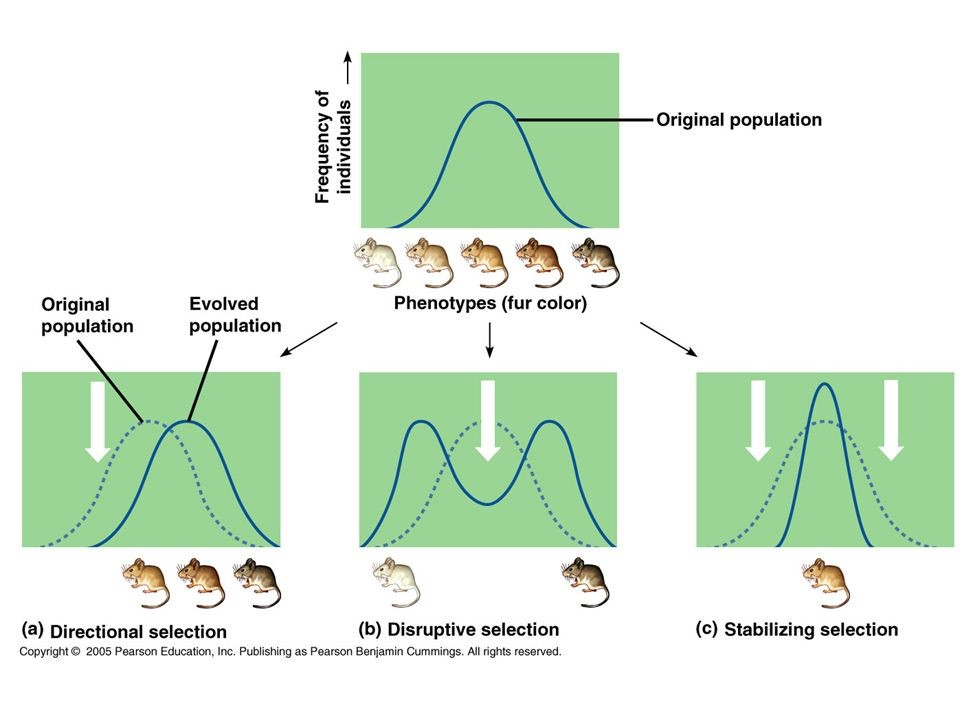
\includegraphics[width=10cm, center]{natural-selection.jpg}
\caption{天擇的方向} \vskip 10 pt
\label{fig:natural-selection}
\end{figure}
\noindent
\begin{enumerate}
\item \textbf{你覺得哪一種天擇最常發生?} \\
\item \textbf{為什麼當談到微演化時,我們都說是「基因」頻率,卻又說天擇偏好的是「表現型」?} \\
\item \textbf{要怎麼觀察一個族群的演化?} \\
\end{enumerate}


\section{哈溫法則}
在理想族群中經過多個世代交替後,基因型頻率會保持恆定且穩定的平衡狀態。 \\

理想族群:
\begin{enumerate}
\item 沒有\underline{\hspace{4em}}發生。
\item 沒有個體的\underline{\hspace{4em}}或\underline{\hspace{4em}}。
\item 族群\underline{\hspace{4em}}。
\item 族群內隨機交配,每一種基因有同等機會傳到後代。
\item 在族群延續過程中,對偶基因(基因組)均相同。
\end{enumerate}

\noindent
例:顯性等位基因記為A而隱性等位基因記為a,它們的頻率分別記為p和q。(記為$f(A) = p, f(a) = q$)。則得知$p + q = 1$ \\
如果群體處於平衡狀態,那我們可以得到:\\
群體中純合子AA的頻率$f(AA) = p^2$ \\
群體中純合子aa的頻率$f(aa) = q^2$ \\
群體中雜合子Aa的頻率$f(Aa) = 2pq$ \\

\begin{figure}[H]
\graphicspath{{biology/}}
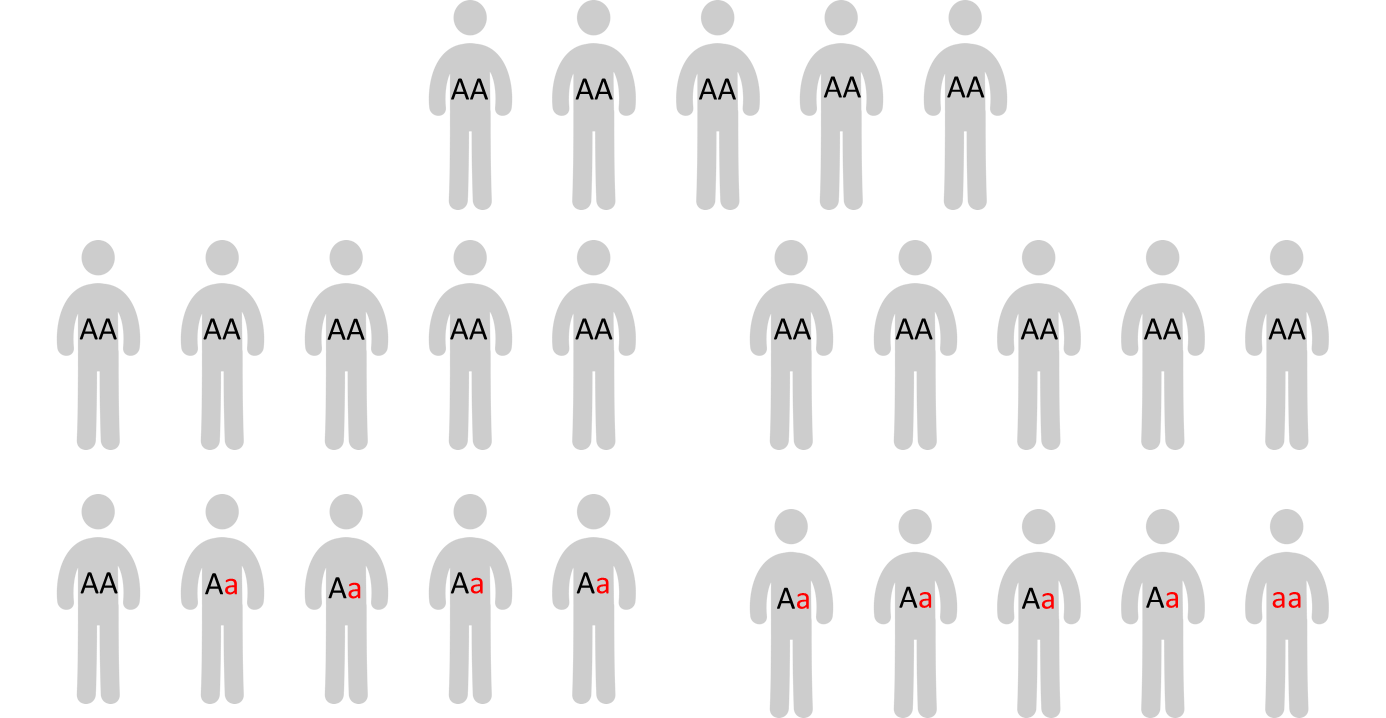
\includegraphics[width=\textwidth, center]{genetic.png}
\caption{等位基因的遺傳} \vskip 10 pt
\label{fig:genetic}
\end{figure}

依性狀由A跟a控制,25人中,有1個隱性性狀者(aa),則: \\
$$q^2 = \frac{1}{25} = 0.04 \rightarrow q=0.2, p=0.8 $$ \\
則推知:
\begin{table}[H]
\centering
\begin{tabular}{|c|c|c|}
\hline
基因型 & 比例          & 人數               \\ \hline
AA  & $(0.8)^2$      & $0.64 \times 25 = 16$ 人 \\ \hline
aa  & $(0.2)^2$      & $0.04 \times 25 = 1$  人 \\ \hline
Aa  & $2(0.8)(0.2)$ & $0.32 \times 25 = 8$  人  \\\hline
\end{tabular}
\end{table}

\noindent
\fbox{小練習}

在一族群中,某基因座有兩種等位基因,16人的基因型為AA,60人為Aa,24人為aa,請用哈溫法則檢視此基因是否在演化。

\section{講師介紹}
\begin{itemize}
\item 姓名:高語儂
\item 性別:女
\item 特色:自己的想法很多、熟捻多國語言、曾任班長但在連任選舉中慘敗、其兄目前就讀香港大學財金系大一,並以學測滿級分(是75喔不是60)同時錄取台大電機系,但講師本人並無特別成就、其父曾經指導國際數學奧林匹亞之選手(編按:詳請請洽講師)...
\item 名言:雪豹好可愛!!!、我哥超認真準備科學班結果沒上,然後我根本沒準備就上了(編按:科學班有單一性別保障6位)。
\end{itemize}

\begin{figure}[H]
\graphicspath{{biology/}}
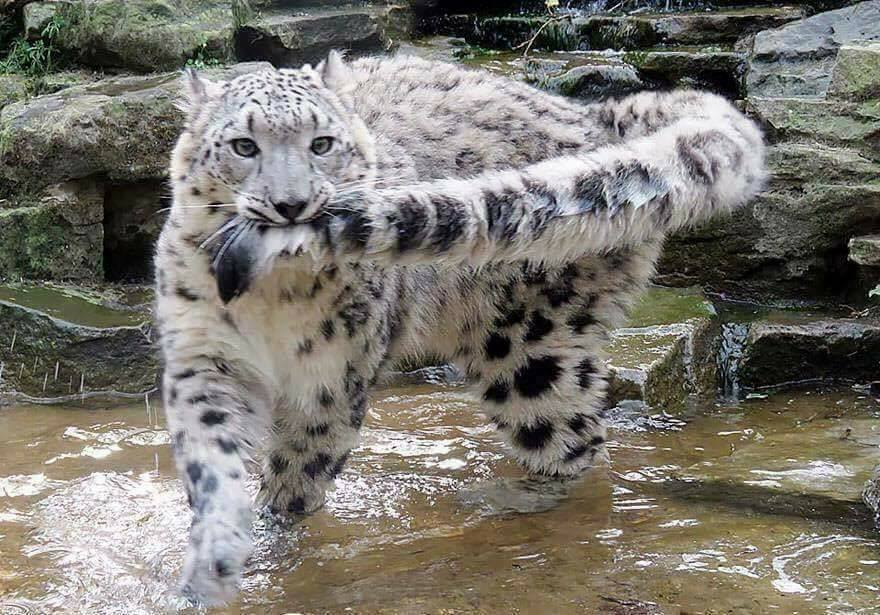
\includegraphics[width=12cm, center]{snowLeopard.jpg}
\caption{講師的最愛:雪豹咬尾巴} \vskip 10 pt
\label{fig:snowLeopard}
\end{figure}